\documentclass[11pt,a4paper]{article}
\usepackage[T1]{fontenc}
\usepackage{lmodern}
\usepackage{geometry}
\geometry{margin=23mm}
\usepackage{microtype}
\usepackage{amsmath,amssymb}
\usepackage{booktabs,longtable,array,tabularx}
\usepackage{enumitem}
\usepackage{xcolor}
\usepackage{listings}
\usepackage{tikz}
\usetikzlibrary{arrows.meta,positioning,shapes.geometric,calc,fit}
\usepackage{hyperref}
\usepackage{fancyhdr}
\usepackage{caption}
\usepackage{float}
\usepackage{parskip}

\definecolor{codebg}{RGB}{247,248,250}
\definecolor{codeframe}{RGB}{210,214,220}
\definecolor{commentgreen}{RGB}{0,105,68}
\definecolor{keywordblue}{RGB}{25,70,155}
\definecolor{stringred}{RGB}{150,35,35}

\lstdefinestyle{cstyle}{
  language=C,
  basicstyle=\ttfamily\small,
  keywordstyle=\color{keywordblue}\bfseries,
  commentstyle=\color{commentgreen}\itshape,
  stringstyle=\color{stringred},
  backgroundcolor=\color{codebg},
  frame=single,
  rulecolor=\color{codeframe},
  numbers=left,
  numberstyle=\tiny\color{gray},
  numbersep=8pt,
  showstringspaces=false,
  tabsize=4,
  breaklines=true,
  columns=fullflexible,
  keepspaces=true,
  captionpos=b
}

\setlist[itemize]{topsep=3pt,itemsep=2pt}
\setlist[enumerate]{topsep=3pt,itemsep=3pt}
\setlength{\headheight}{14pt}
\setlength{\parindent}{0pt}
\emergencystretch=2em

\pagestyle{fancy}
\fancyhf{}
\lhead{SmartSafe Project}
\rhead{Tamper Detection Module}
\cfoot{\thepage}

\hypersetup{
  colorlinks=true,
  linkcolor=blue!60!black,
  urlcolor=blue!60!black,
  pdftitle={SmartSafe Tamper Detection Module},
  pdfauthor={Microprocessors End-Term Project}
}

\title{\textbf{SmartSafe Master Unit}\\[4pt]
\Large Complete Design and Code Explanation of the ADC Tamper-Detection Module}
\author{Microprocessors End-Term Project}
\date{July 2026}

\begin{document}
\maketitle
\thispagestyle{empty}

\begin{abstract}
This report documents the SmartSafe tamper-detection subsystem. A potentiometer connected to \texttt{PA3/ADC3} simulates displacement, vibration, or impact. The ATmega32 ADC converts the analog wiper voltage into a 10-bit sample approximately every 100 ms. The report explains the sensor wiring, why the pin is an input with its internal pull-up disabled, the \texttt{ADMUX} and \texttt{ADCSRA} register settings, AVCC reference selection, ADC clock and conversion-time calculations, voltage resolution, the choice of a 50-count threshold, Timer2 CTC calculations, the difference between consecutive-sample and stable-reference detection, event rearming, main-loop integration, USART notification and the 9600-baud calculation, external EEPROM logging, sleep and power-restoration behavior, and detailed Proteus testing and troubleshooting.
\end{abstract}

\tableofcontents
\newpage

\section{Purpose of the Tamper Subsystem}
The project specification requires periodic monitoring of a simulated vibration or impact sensor and an alarm when the sensor changes suddenly beyond a threshold. In Proteus, a potentiometer represents this sensor. The Master performs detection and sends an event to the independently powered Slave. The Slave owns the red LED, buzzer driver, and alarm LCD message.

A new tamper event causes the Master to:
\begin{enumerate}
  \item transmit \texttt{Tamper\textbackslash r\textbackslash n} through USART;
  \item store \texttt{EVT\_TAMPER} with a timestamp in the external SPI EEPROM;
  \item block keypad input for five seconds without replacing the Master password prompt;
  \item reset the inactivity counter so the Master does not immediately sleep.
\end{enumerate}

\section{Hardware Connection}
The potentiometer is connected as a voltage divider:
\begin{center}
\begin{tabular}{ll}
\toprule
Potentiometer terminal & Connection \\
\midrule
Upper end & +5 V \\
Lower end & GND \\
Wiper & PA3/ADC3 \\
\bottomrule
\end{tabular}
\end{center}

\begin{figure}[H]
\centering
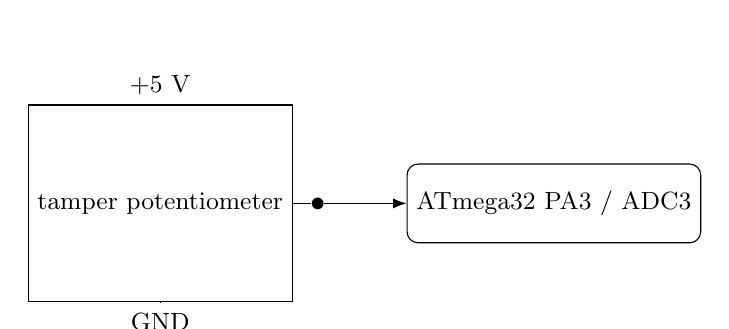
\begin{tikzpicture}[>=Latex,every node/.style={font=\small}]
\node (vcc) at (0,3.0) {+5 V};
\node[draw,minimum width=18mm,minimum height=25mm] (pot) at (0,1.5) {tamper potentiometer};
\node (gnd) at (0,0) {GND};
\node[circle,fill=black,inner sep=1.5pt] (wiper) at (2.0,1.5) {};
\node[draw,rounded corners,minimum width=34mm,minimum height=10mm] (adc) at (5.0,1.5) {ATmega32 PA3 / ADC3};
\draw (vcc) -- (pot.north);
\draw (pot.south) -- (gnd);
\draw[->] (pot.east) -- (wiper) -- (adc.west);
\end{tikzpicture}
\caption{Tamper potentiometer and ADC3 connection.}
\end{figure}

The analog supply requirements are:
\begin{itemize}
  \item \texttt{AVCC} connected to +5 V;
  \item both MCU grounds connected to GND;
  \item \texttt{AREF} bypassed to ground with approximately 100 nF when AVCC is used as the reference;
  \item no direct short from AREF to ground;
  \item the potentiometer and MCU share the same ground.
\end{itemize}

\section{Why the Internal Pull-Up Is Disabled}
The ADC pin is configured as an input and its pull-up is disabled:
\begin{lstlisting}[style=cstyle]
ADC_TAMPER_DDR  &= ~(1U << ADC_TAMPER_PIN);
ADC_TAMPER_PORT &= ~(1U << ADC_TAMPER_PIN);
\end{lstlisting}
For an AVR pin, \texttt{DDRx=0} selects input. With input selected, \texttt{PORTx=1} would connect a weak internal resistor to VCC. That resistor would become part of the external potentiometer network, pull the wiper voltage upward, and distort the ADC result. The potentiometer already gives the pin a defined analog voltage, so no digital bias resistor is needed.

This is different from keypad columns, where an internal pull-up is intentionally used to define the idle state of an otherwise disconnected digital switch input.

\section{ADC Register Configuration}
The initialization code is:
\begin{lstlisting}[style=cstyle,caption={ADC initialization for the tamper sensor.}]
void adc_init(void)
{
    ADC_TAMPER_DDR  &= ~(1U << ADC_TAMPER_PIN);
    ADC_TAMPER_PORT &= ~(1U << ADC_TAMPER_PIN);

    ADMUX  = (1U << REFS0);
    ADCSRA = (1U << ADEN) |
             (1U << ADPS2) |
             (1U << ADPS1);
}
\end{lstlisting}

\subsection{ADMUX configuration}
The relevant fields are:
\begin{center}
\begin{tabular}{cll}
\toprule
Field & Value & Result \\
\midrule
REFS1:REFS0 & 01 & AVCC used as ADC reference \\
ADLAR & 0 & Conversion result right-adjusted \\
MUX4:0 at initialization & 00000 & Channel selected later by \texttt{adc\_read()} \\
\bottomrule
\end{tabular}
\end{center}
With \texttt{REFS0=1} and \texttt{REFS1=0}, the conversion range is nominally 0 V to AVCC. The AREF pin is used for decoupling the selected internal reference path.

Right adjustment allows the complete 10-bit result to be read conveniently through the AVR-GCC \texttt{ADC} 16-bit register macro.

\subsection{ADCSRA configuration}
\begin{center}
\begin{tabular}{clp{0.52\textwidth}}
\toprule
Bit & Value & Purpose \\
\midrule
ADEN & 1 & Enable the ADC peripheral. \\
ADSC & 0 at initialization & A conversion is started later by software. \\
ADATE & 0 & Disable auto-trigger; use single conversions. \\
ADIF & 0 & Conversion-complete flag not used for interrupt operation. \\
ADIE & 0 & ADC interrupt disabled; the driver polls completion. \\
ADPS2:0 & 110 & Prescaler 64. \\
\bottomrule
\end{tabular}
\end{center}

\section{ADC Clock Calculation}
The CPU clock is 8 MHz. With prescaler 64:
\[
f_{ADC}=\frac{8\,000\,000}{64}=125\,000\text{ Hz}=125\text{ kHz}.
\]
One ADC clock period is
\[
T_{ADC}=\frac{1}{125\,000}=8\ \mu\text{s}.
\]
A normal single conversion requires approximately 13 ADC clock cycles, so its approximate conversion time is
\[
13\times8=104\ \mu\text{s}.
\]
The first conversion after enabling the ADC requires additional initialization cycles and is longer, approximately 25 ADC clocks or 200 microseconds. This is still much shorter than the 100 ms sampling interval.

The 125 kHz ADC clock is chosen because it is within the range conventionally recommended for full 10-bit accuracy on classic AVR devices, while remaining fast enough for this low-frequency sensor.

\section{Channel Selection and Conversion Procedure}
The read function is:
\begin{lstlisting}[style=cstyle,caption={Single-channel ADC read.}]
uint16_t adc_read(uint8_t channel)
{
    ADMUX = (ADMUX & 0xE0U) | (channel & 0x07U);

    ADCSRA |= (1U << ADSC);
    while (ADCSRA & (1U << ADSC)) {
        /* wait for hardware to clear ADSC */
    }

    return ADC;
}
\end{lstlisting}

For the tamper sensor, \texttt{channel=3}, so the multiplexer bits become \texttt{00011}, selecting PA3/ADC3. The mask preserves the reference-selection and result-alignment bits.

The sequence is:
\begin{enumerate}
  \item select ADC3 in \texttt{ADMUX};
  \item set \texttt{ADSC} to start conversion;
  \item wait while \texttt{ADSC} remains one;
  \item hardware clears \texttt{ADSC} when conversion finishes;
  \item read the 10-bit result.
\end{enumerate}

On the 8-bit AVR bus, the low result byte must be read before the high byte. The compiler-provided \texttt{ADC} macro performs the correct ordered access for a 16-bit result.

\section{ADC Resolution and Threshold Calculation}
For a 10-bit ADC, output codes range from 0 through 1023. With a nominal 5 V reference, one least-significant bit represents approximately
\[
V_{LSB}=\frac{5}{1024}=4.8828\text{ mV}.
\]
The selected threshold is:
\begin{lstlisting}[style=cstyle]
#define TAMPER_THRESHOLD 50U
\end{lstlisting}
Its voltage equivalent is approximately
\[
50\times4.8828\text{ mV}=244.14\text{ mV}.
\]
A 50-count change is large enough to reject minor quantization noise and small simulation fluctuations, yet small enough to respond to deliberate potentiometer movement.

If AVCC differs from exactly 5 V, the voltage represented by one count changes proportionally. The algorithm is fundamentally based on ADC counts, so its effective voltage threshold tracks the reference voltage.

\section{Periodic Sampling with Timer2}
The ADC is sampled when Timer2 produces a 100 ms software flag. Timer2 is configured in CTC mode with:
\begin{lstlisting}[style=cstyle]
OCR2 = 77U;
TIMSK |= (1U << OCIE2);
TCCR2 = (1U << WGM21) |
        (1U << CS22)  |
        (1U << CS21)  |
        (1U << CS20);
\end{lstlisting}
The prescaler is 1024 and the compare period is
\[
T_{match}=\frac{1024(77+1)}{8\,000\,000}=9.984\text{ ms}.
\]
Ten matches produce approximately 99.84 ms. The ISR sets \texttt{timer\_tick\_100ms=1}; the main loop clears it and performs one ADC sample.

The ADC conversion itself takes only about 104 microseconds, approximately 0.1 percent of the 100 ms interval. Therefore periodic tamper sampling has negligible CPU cost.

\section{Detection Algorithms}
\subsection{Earlier consecutive-sample method}
A simple implementation calculates
\[
difference=|sample_{n}-sample_{n-1}|.
\]
It works well for a sudden step. However, gradual manual movement can be missed. For example:
\[
500,510,520,530,540,550
\]
has a total movement of 50 counts, but every consecutive difference is only 10 counts.

\subsection{Recommended stable-reference method}
The final recommended method compares the current sample with a stable reference that is not replaced during ordinary armed monitoring. Several small movements therefore accumulate relative to the baseline.

\begin{lstlisting}[style=cstyle,caption={Robust stable-reference tamper detector.}]
#define TAMPER_REARM_BAND       5U
#define TAMPER_STABLE_SAMPLES   3U

static uint16_t reference_adc = 0U;
static uint8_t armed = 1U;
static uint8_t stable_samples = 0U;

static uint16_t adc_difference(uint16_t a, uint16_t b)
{
    return (a >= b) ? (a - b) : (b - a);
}

void tamper_init(void)
{
    reference_adc = adc_read(ADC_TAMPER_CH);
    armed = 1U;
    stable_samples = 0U;
}

uint8_t tamper_check(void)
{
    uint16_t value = adc_read(ADC_TAMPER_CH);
    uint16_t difference = adc_difference(value, reference_adc);

    if (armed) {
        if (difference > TAMPER_THRESHOLD) {
            armed = 0U;
            stable_samples = 0U;
            reference_adc = value;
            return 1U;
        }
        return 0U;
    }

    if (difference <= TAMPER_REARM_BAND) {
        if (++stable_samples >= TAMPER_STABLE_SAMPLES) {
            armed = 1U;
            stable_samples = 0U;
        }
    } else {
        reference_adc = value;
        stable_samples = 0U;
    }

    return 0U;
}
\end{lstlisting}

\section{Initialization and Baseline Selection}
\texttt{tamper\_init()} performs an ADC conversion and uses the present potentiometer position as the initial reference. This prevents startup from being interpreted as tampering merely because the source code chose a fixed default such as 512 while the actual potentiometer starts elsewhere.

The same initialization is performed after power-restoration reinitialization. The new stable physical position becomes the baseline after the Master returns from power-failure standby.

\section{Arming and Rearming}
After a threshold crossing, the detector returns exactly one event and becomes disarmed. Without this state, a displaced potentiometer could generate a new event every 100 ms.

The rearm logic requires three consecutive readings within five ADC counts of the current reference:
\[
5\text{ counts}\times4.8828\text{ mV}\approx24.4\text{ mV}.
\]
Three 100 ms samples require approximately 300 ms of stability. This gives the simulated sensor time to settle before a new event can be accepted.

When the sensor continues moving while disarmed, the reference follows the latest value and the stability counter restarts. Once motion stops, the stable-sample requirement is satisfied and the detector rearms at the new resting position.

\section{Main-Loop Integration}
The relevant main-loop structure is:
\begin{lstlisting}[style=cstyle]
if (timer_tick_100ms) {
    uint32_t now;
    timer_tick_100ms = 0U;

    if (tamper_check()) {
        now = timer_get_seconds();
        usart_print(MSG_TAMPER);
        log_event(EVT_TAMPER, now);

        ui_hold_until = now + TAMPER_UI_HOLD_SEC;
        activity_timer = 0U;
    }
}
\end{lstlisting}
The low-level detector only returns a Boolean event. It does not call the LCD, USART, logger, or alarm outputs. This separation keeps the sensor module reusable and keeps system policy in \texttt{main.c}.

\section{USART Notification and Baud-Rate Calculation}
The tamper message is:
\begin{lstlisting}[style=cstyle]
#define MSG_TAMPER "Tamper\r\n"
\end{lstlisting}
The project uses normal asynchronous USART mode at 9600 baud with an 8 MHz CPU clock. The UBRR equation is
\[
UBRR=\frac{F_{CPU}}{16\times Baud}-1.
\]
Therefore
\[
UBRR=\frac{8\,000\,000}{16\times9600}-1=51.0833.
\]
The nearest integer is 51. The actual baud rate is
\[
Baud_{actual}=\frac{8\,000\,000}{16(51+1)}=9615.38\text{ baud}.
\]
The error is
\[
\frac{9615.38-9600}{9600}\times100\approx0.16\text{ percent}.
\]

The USART configuration is:
\begin{lstlisting}[style=cstyle]
UBRRH = 0U;
UBRRL = 51U;
UCSRB = (1U << RXEN) | (1U << TXEN);
UCSRC = (1U << URSEL) |
        (1U << UCSZ1) |
        (1U << UCSZ0);  /* 8 data, no parity, 1 stop */
\end{lstlisting}
The string \texttt{Tamper\textbackslash r\textbackslash n} contains eight characters. In 8N1 format each character occupies ten serial bits: one start, eight data, and one stop. Its approximate transmission time is therefore
\[
\frac{8\times10}{9600}=8.33\text{ ms}.
\]
This is much shorter than the 100 ms sensor interval and is adequate for remote alarm notification.

\section{Event Logging}
After transmission, the Master stores \texttt{EVT\_TAMPER} and the current seconds timestamp in the 25LC040 SPI EEPROM. Logging is performed outside the ADC routine so that analog acquisition remains independent from the storage protocol. The external EEPROM record survives reset and can later be dumped through the virtual terminal.

The logger and USART operations may take several milliseconds, but the detector is disarmed immediately after the event. Therefore the same disturbance does not produce repeated entries while the notification is being processed.

\section{Master and Slave Responsibilities}
\begin{center}
\begin{tabularx}{\textwidth}{p{0.27\textwidth}X}
\toprule
Unit & Responsibility \\
\midrule
Master & Sample ADC3, evaluate threshold, timestamp and log event, send \texttt{Tamper}, block keypad temporarily. \\
Slave & Match the received message, display the tamper warning, activate the red LED and buzzer driver for the required duration. \\
\bottomrule
\end{tabularx}
\end{center}
The Master has no local alarm LED or buzzer in the final design.

\section{Interaction with Sleep and Power Failure}
\subsection{Normal inactivity Power-down}
When the Master enters inactivity Power-down, Timer2 and the ADC stop. Moving the tamper potentiometer cannot wake the Master. The INT0 wake button must first wake normal operation, after which periodic ADC sampling resumes.

\subsection{Power-failure standby}
After a confirmed monitored power failure, the Master disables the ADC and Timer2. Only the analog comparator remains as the restoration wake source. After restoration, the runtime initialization sequence reenables ADC3, reads a new tamper baseline, restarts Timer2, and resumes monitoring.

\section{Timing and Constant Summary}
\begin{longtable}{p{0.29\textwidth}p{0.22\textwidth}p{0.41\textwidth}}
\toprule
Item & Value & Reason \\
\midrule
\endhead
CPU clock & 8 MHz & Common project clock and convenient peripheral calculations. \\
ADC reference & AVCC, nominal 5 V & Full potentiometer range corresponds to ADC codes 0--1023. \\
ADC prescaler & 64 & Produces 125 kHz ADC clock. \\
Normal conversion time & about 104 microseconds & 13 ADC clocks at 125 kHz. \\
ADC resolution & about 4.883 mV/count & 5 V divided by 1024. \\
Tamper threshold & 50 counts & Approximately 244 mV; rejects small noise. \\
Timer2 prescaler & 1024 & Allows an approximately 10 ms compare interval with an 8-bit timer. \\
\texttt{OCR2} & 77 & 78 counts produce 9.984 ms. \\
Sampling interval & about 99.84 ms & Ten Timer2 compare matches. \\
Rearm band & 5 counts & Approximately 24.4 mV stability band. \\
Stable samples & 3 & Approximately 300 ms before rearming. \\
USART UBRR & 51 & Actual baud approximately 9615, error 0.16 percent. \\
Tamper UI hold & 5 s & Matches the ordinary remote alarm interval. \\
\bottomrule
\end{longtable}

\section{Proteus Test Procedure}
\begin{enumerate}
  \item Set the Master ATmega32 clock property to 8 MHz.
  \item Connect the potentiometer ends to +5 V and GND and the wiper to PA3/ADC3.
  \item Connect AVCC to +5 V and place a capacitor from AREF to ground.
  \item Wake the Master and confirm the password prompt is active.
  \item Note the initial potentiometer position; it becomes the baseline.
  \item Move the wiper enough to exceed approximately 50 ADC counts.
  \item Confirm the Master sends \texttt{Tamper} and stores one event.
  \item Confirm the Slave displays the tamper status and activates its alarm.
  \item Hold the potentiometer at the new position; no repeated event should occur.
  \item Keep it stable for at least about 300 ms, then move it again to test rearming.
\end{enumerate}

For diagnosis, the ADC result can be temporarily printed to the terminal or watched in the debugger. At 0 V it should be near 0, near half supply it should be around 512, and near 5 V it should approach 1023.

\section{Common Failure Modes}
\begin{longtable}{p{0.31\textwidth}p{0.61\textwidth}}
\toprule
Symptom & Likely cause and correction \\
\midrule
\endhead
ADC always reads zero & AVCC is not powered, AREF is incorrectly shorted, the wiper is not connected to PA3, or ADC is disabled. \\
ADC always reads near 1023 & Pull-up is enabled on PA3, wiper is tied to VCC, or lower potentiometer terminal is not grounded. \\
Slow movement does not trigger & Consecutive-sample algorithm is still used; use the stable-reference algorithm. \\
Repeated events every 100 ms & Detector is not disarmed after the first event or rearm logic is missing. \\
No event after ten seconds & Master entered Power-down; wake it with INT0 before testing. \\
Tamper works on Master but not Slave & USART wiring, common ground, 9600 8N1 settings, or exact message matching is wrong. \\
False event immediately at startup & Fixed baseline was used instead of reading the actual startup ADC value. \\
Tamper stops after power restoration & ADC, Timer2, or \texttt{tamper\_init()} was not reinitialized. \\
\bottomrule
\end{longtable}

\section{Conclusion}
The tamper subsystem combines a simple analog sensor simulation with deterministic digital processing. ADC3 is configured with AVCC reference, right-adjusted 10-bit results, and a /64 prescaler that produces a 125 kHz ADC clock. Timer2 schedules a sample every approximately 100 ms. A 50-count threshold corresponds to about 244 mV at a 5 V reference. The stable-reference and rearm state machine detects both sudden and accumulated displacement while preventing duplicate alarms. USART then transports the event at 9600 baud and the external EEPROM preserves it for later inspection.

\begin{thebibliography}{9}
\bibitem{atmega}
Microchip Technology Inc., \emph{ATmega32A Data Sheet}, sections on ADC, Timer/Counter2, USART, I/O ports, and sleep modes.\\
\href{https://ww1.microchip.com/downloads/en/DeviceDoc/Atmega32A-Data-Sheet-DS40002072A.pdf}{Official Microchip PDF}

\bibitem{avr042}
Microchip Technology Inc., \emph{AVR042: AVR Hardware Design Considerations}, analog supply, reference, and decoupling guidance.\\
\href{https://ww1.microchip.com/downloads/en/AppNotes/Atmel-2521-AVR-Hardware-Design-Considerations_ApplicationNote_AVR042.pdf}{Official Microchip application note}

\bibitem{project}
Microprocessors End-Term Project, \emph{Smart Safe with Remote Alarm}, project specification supplied with the implementation.

\bibitem{source}
SmartSafe source files: \texttt{adc.c}, \texttt{tamper.c}, \texttt{timer.c}, \texttt{usart.c}, \texttt{config.h}, and \texttt{main.c}, July 2026 project version.
\end{thebibliography}

\end{document}
